\documentclass[12pt]{book}
\usepackage[a4paper, total={6in, 8in}]{geometry}
\usepackage{amssymb}
\usepackage{listings}
\usepackage{color}
\usepackage{graphicx}
\usepackage{subfig}
\usepackage{float}
\definecolor{mygrey}{gray}{.96} % Light Grey
\definecolor{BrickRed}{RGB}{120,0,0}


\def\xbf{\mathbf{x}}
\def\zbf{\mathbf{z}}
\def\xibf{\mathbf{\xi}}
\lstset{
	language=C++,              % choose the language of the code ("language=Verilog" is popular as well)
   tabsize=3,							  % sets the size of the tabs in spaces (1 Tab is replaced with 3 spaces)
	basicstyle=\footnotesize,               % the size of the fonts that are used for the code
	numbers=left,                   % where to put the line-numbers
	numberstyle=\footnotesize,              % the size of the fonts that are used for the line-numbers
	stepnumber=1,                   % the step between two line-numbers. If it's 1 each line will be numbered
	numbersep=5pt,                  % how far the line-numbers are from the code
	backgroundcolor=\color{mygrey}, % choose the background color. You must add \usepackage{color}
	showspaces=false,              % show spaces adding particular underscores
	showstringspaces=false,        % underline spaces within strings
	showtabs=false,                % show tabs within strings adding particular underscores
	frame=single,	                 % adds a frame around the code
	tabsize=3,	                    % sets default tabsize to 2 spaces
	captionpos=b,                   % sets the caption-position to bottom
	breaklines=true,                % sets automatic line breaking
	breakatwhitespace=false,        % sets if automatic breaks should only happen at whitespace
	%escapeinside={\%*}{*)},        % if you want to add a comment within your code
	commentstyle=\color{BrickRed}   % sets the comment style
}

\begin{document}
\title{\textbf{Monte Carlo Simulation Lab\\Assignment-6}}	
\author{Yash Vanjani\\(140123046)\\Mathematics and Computing\\IIT Guwahati}
\date{March 15th, 2016}

\maketitle

\newpage
\begin{enumerate}
\item[Q 1] Generate 50 randam numbers from geometric distribution of the form :
$$f (x; p) = pq^{i-1} , i = 1, 2, . . . , 0 < p < 1$$
Draw the probability mass function.
\end{enumerate}
\noindent{Code for R :}

\begin{lstlisting}
U<-runif(50)
X<-vector("numeric")
p=0.123
q=1-p
for(i in 1:50)
{
	X[i]=(floor(log(U[i])/log(q))+1)
}
print(X)
frequency<-array(0,50)
for (i in 1:50) 
{
	frequency[X[i]]=frequency[X[i]]+1
}
print(frequency)
probability<-array(0,50)
for (i in 1:50)
{
	probability[i]=frequency[i]/50
}
print(probability)
png("assign6q1.png")
hist(X,col="red",main=paste("pmf of Geometric distribution(",p,",",q,")"),xlab="X",ylab="Probability", freq=FALSE, breaks=15)
\end{lstlisting}
\newpage
The probability mass function is as follows for 50 values:
\begin{figure}[H]
	\centering
	\subfloat[Probability mass function]{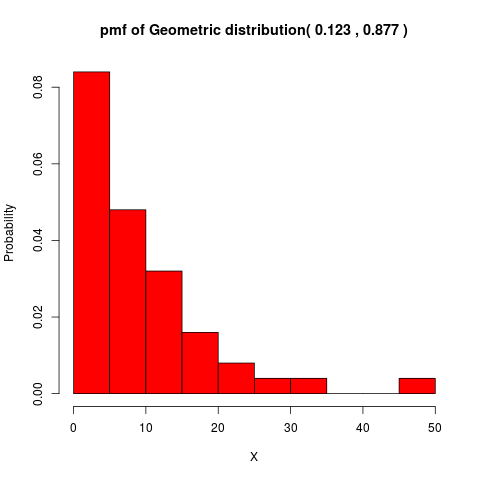
\includegraphics[width=1\textwidth]{assign6q1.png}}	
\end{figure}
\newpage
\begin{enumerate}
\item[Q 2] Generate 50 random numbers from poisson distribution with mean 2. Draw the probability mass function and the cumulative distribution function.
\end{enumerate}
\noindent{Code for R: }
\begin{lstlisting}
f<-function()
{
	u<-runif(50)
	v<-array(50);
	for(j in 1:50)
	{
		i=0;
		p=exp(-2);
		f=p;
		while(u[i]>f)
		{
			p=2*p/(i+1);
			f=f+p;
			i=i+1;
		}
		v[j]=i;
	}
	print(v)
	png("assign6q2.png");
	hist(v,freq=F,col="red");
	dev.off();
	png("assign6q2cdf.png");
	plot(ecdf(v),col="red");
	dev.off();
}
\end{lstlisting}
\newpage
The probability mass function is as follows:\\\\
\begin{figure}[H]
	\centering
	\subfloat[Probability mass function]{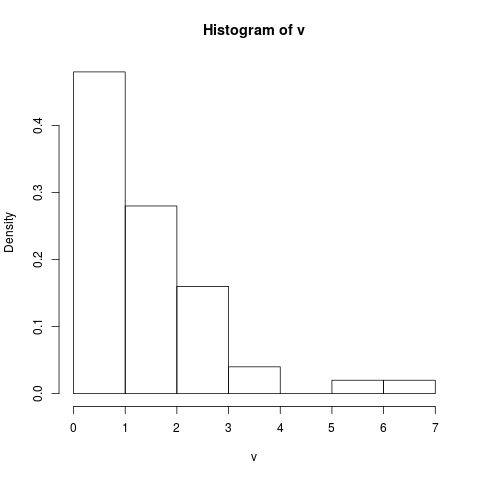
\includegraphics[width=1\textwidth]{assign6q2.png}}	
\end{figure}
\newpage
The cumulative density function is as follows: \\
\begin{figure}[H]
	\centering
	\subfloat[Cumulative density function]{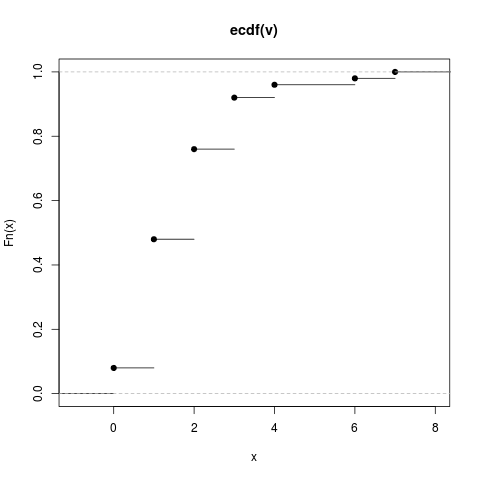
\includegraphics[width=1\textwidth]{assign6q2cdf.png}}	
\end{figure}
\newpage
\begin{enumerate}
\item[Q 3] Draw the histogram based 50 generated random numbers from the mixture of
two Weibull distributions :
$$f (x; \beta_1 , \theta_1 , \beta_2 , \theta_2 , p) = p*f_1 (x; \beta_1 , \theta_1 ) + (1-p)*f_2 (x; \beta_2 , \theta_2 )$$
where $f_1 ()$ and $f_2 ()$ are two Weibull distributions of the form:\\ $$f (x; \beta, \theta) =
\beta \theta^\beta x^{\beta-1} e^{−(\theta x)}$$ \\where, $\beta_1 = 2, \theta_1 = 1, \beta_2 = 1.5, \theta_2 = 1, p = 0.4$.
\end{enumerate}
\noindent{Code for R :}\\
\begin{lstlisting}
u<-runif(50)
f<-array(0,50)
x1<-array(0,50)
x2<-array(0,50)
for(i in 1:50)
{
	x1[i]=rweibull(1,2,1)
	x2[i]=rweibull(1,1.5,1)
	if(u[i]<=0.4)
		f[i]=x1[i]
	if(u[i]>0.4)
		f[i]=x2[i]
}
print(f)
png("assign6q3.png")
hist(f,col="red")
\end{lstlisting}
\newpage
The histogram formed is as follows: \\
\begin{figure}[H]
	\centering
	\subfloat[Histogram]{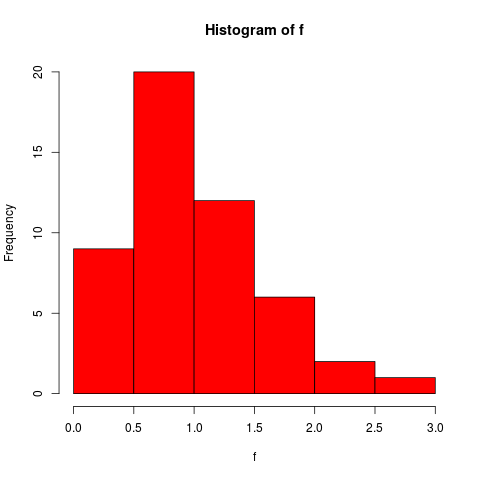
\includegraphics[width=1\textwidth]{assign6q3.png}}	
\end{figure}



\end{document}